%!TEX root = ../thesis.tex

\subsection{グラフ探索}

\begin{figure}[hbtp]
  \centering
 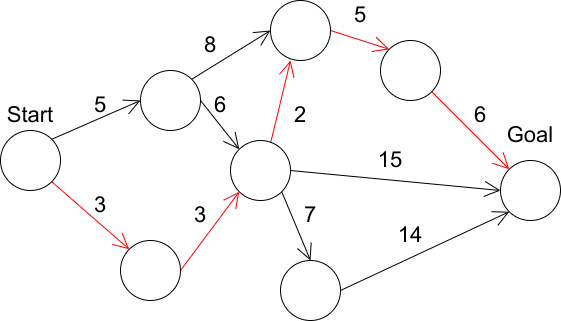
\includegraphics[keepaspectratio, scale=0.6]
      {images/png/Dijkstra.drawio.png}
 \caption{Connected graph}
 \label{Fig:Dijkstra}
\end{figure}

グラフ探索では,経由する点と点を結び最短な経路を探索する.
ここで点を「頂点」,点と点を結んで線にしたものを「パス」という.
グラフ探索ベースの経路計画では,
スタートの距離,すなわち重みを0として頂点間のパスに指定された重みに応じて頂点の重みが加算されていく.
最終的にゴールまでの重みが小さい経路が選択されそれが最短の経路であるという理論である.
Fig.\ref{Fig:Dijkstra}がそのイメージ図である.円が頂点,矢印がパスである.
現実的には,点がロボットが経由する地点で,矢印がロボットが移動する経路で重みがロボットが移動する距離である.
赤い矢印の経路が最も重みが小さいため,最短経路ということになる.

しかし,このアルゴリズムにはパスがロボットの運動として適切かどうかという問題がある.
すなわち,前述したロボットの機構や特性を無視したパスが生成される問題である.
それらの問題があってもスタートからゴールまでを最短距離で移動するには有用なアルゴリズムであり,ダイクストラ法やA*法で使用されている.
これらのアルゴリズムは大域経路計画としても使用されている.

グラフ探索の別の応用先としてはカーナビゲーションが挙げられる.
\newpage
